\documentclass[a4paper, 10pt]{article}

\usepackage[utf8]{inputenc}
\usepackage[scale=0.8]{geometry}
\usepackage{hyperref}
\usepackage{graphicx}

\renewcommand*\contentsname{Table des matières}

\title{\textbf{Manuel d'installation}}
\author{Guardians Studio}
\date{Année scolaire 2021-2022}

\begin{document}
	\maketitle
	\tableofcontents
	\section{Pour installer le launcher}
	Rendez vous sur la page téléchargements de notre site :
	\url{https://guardiansstudio.000webhostapp.com/download.php}.
	Puis scrollez vers le bas jusqu'à voir le bouton de téléchargement du jeu et cliquez dessus pour lancer le téléchargement.
	
	\begin{figure}[ht]
		\centering
		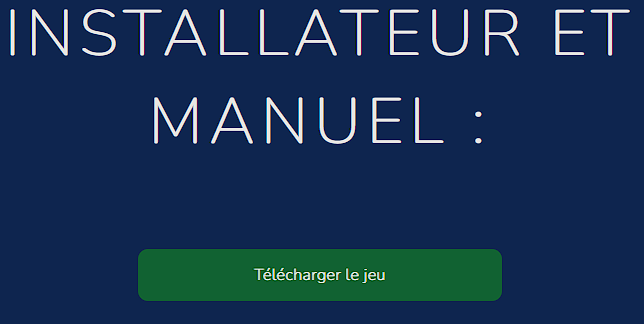
\includegraphics[scale=0.6]{images/download_launcher.png}
		\caption{Bouton de téléchargement du jeu}
	\end{figure}

	\section{Utiliser le launcher}
	
\end{document}